\documentclass[12pt]{article}

% font
\usepackage{lmodern}

% packages
\usepackage[margin=1in, a4paper]{geometry}
\usepackage{indentfirst}
\usepackage{amsmath}
\usepackage{mathtools}
\usepackage{footmisc}
\usepackage{gensymb}
\usepackage{xcolor}
\usepackage{listings}
\usepackage{caption}
\usepackage{sectsty}
\usepackage[colorlinks, allcolors=blue]{hyperref}

% size config of sections
\sectionfont{\fontsize{12}{15}\selectfont}
\subsectionfont{\fontsize{12}{15}\selectfont}
\subsubsectionfont{\fontsize{12}{15}\selectfont}

% paper info
\title{helloworld}
\author{John Doe}
\date{August 06, 2022}

\begin{document}
    \section{Math}

    This program is planned to support the most basic LaTeX features, you can use inline math with $a + b = c^2$. And this will be the paragraph math:

    \begin{equation}
        \oint \boldsymbol{B} \cdot d \boldsymbol{A} = 0
    \end{equation}

    \subsection{Images}

    You can also insert images with:

    \begin{figure}[h]
        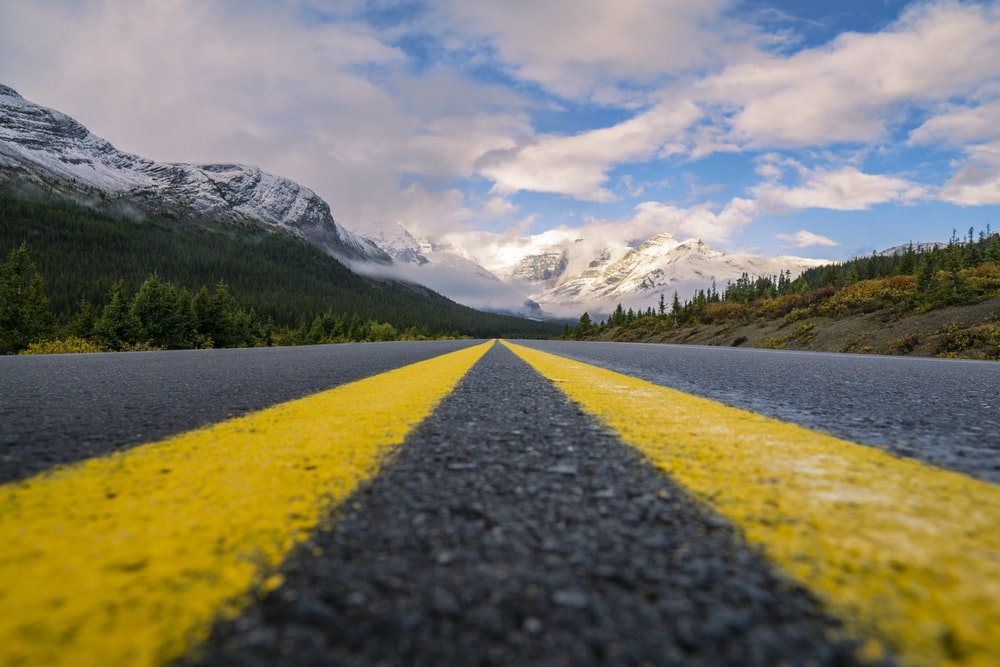
\includegraphics[width=\textwidth]{./sample_image.jpeg}
    \end{figure}

    or by:

    \begin{center}
        \begin{figure}[h]
            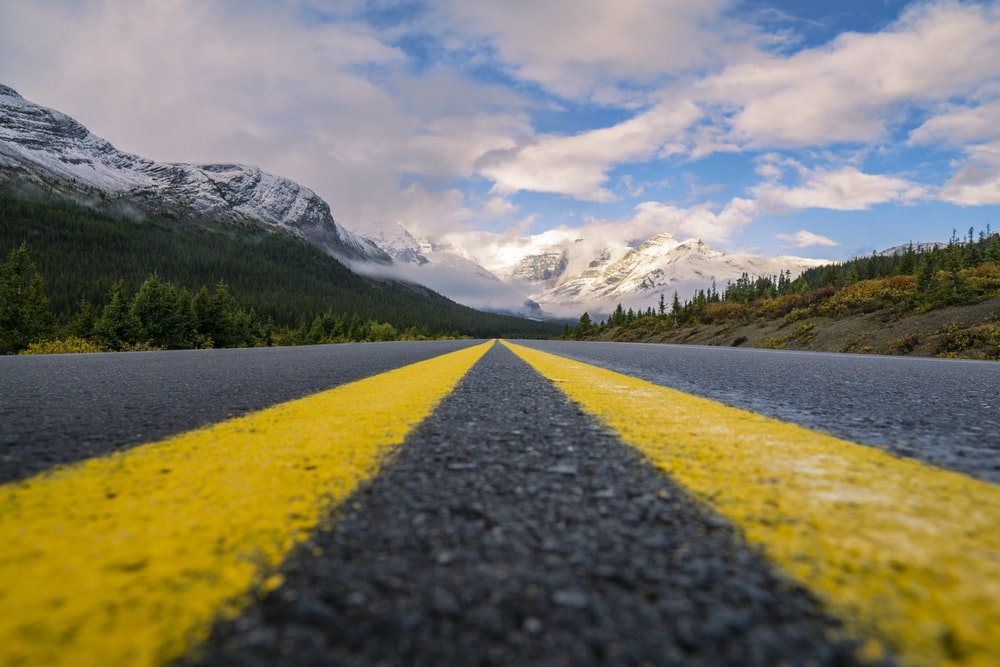
\includegraphics[width=\textwidth]{./sample_image.jpeg}
        \end{figure}
    \end{center}

    \subsubsection{Listings}

    And code blocks with:

\begin{lstlisting}[language=C]
#include <stdio.h>


void say() {
    printf("this is code blocks!");
}


int main() {
    char hello_world[] = "hello world!\n";
    printf(helloworld);

    say();

    return 0;
}
\end{lstlisting}

    \paragraph{This is paragraph}

    Check \href{./example.tex}{example.tex} for the LaTeX rendition of this markdown file. The output of the command is always placed in \texttt{./out/}.

\end{document}
